\documentclass[10pt]{article}
\usepackage{icmlko}

\icmlmeta{IP 파운데이션 월드모델}{140}{전체 상관이 숨긴 하나}{축 이름이 도메인을 건너 같은 뜻인지 처음 쟀다 --- 대개 같았고, 딱 한 쌍이 뒤집혀 있었으며, 그 하나가 노트 138과 139를 전부 설명한다}

\begin{document}

\twocolumn[
\icmlheader

\begin{abstract}
노트 139가 새 질문을 남겼다 --- \texttt{entry\_friction}(입장 마찰)이 웹툰에서
완결 여부와 상관 $-$0.84라면, 축 이름이 도메인을 건너 같은 뜻을 유지하고
있는가? 노트 5 이후 한 번도 안 잰 자리다. 쟀다. \textbf{대개 같다.}
축마다 라벨과의 부호를 도메인 여덟에서 보면 \texttt{target\_breadth}가
8/8 양수, \texttt{media\_push}가 5/5, \texttt{goods\_scale}이 7/7이다.
갈리는 것은 둘 --- \texttt{entry\_friction} 5/7, \texttt{venue\_prominence}
4/7이고 둘 다 $|r|$이 0.12$\sim$0.19로 약하다. \textbf{그런데 전체 상관이
거짓말을 하고 있었다.} 웹툰의 \texttt{entry\_friction}은 전체로 보면
$+$0.019로 무관인데, 2025년 이전 $+$0.129 · 이후 $+$0.301로 \emph{양쪽 다
양수이고 강해진다} --- 두 기간의 수준이 달라 합치면 상쇄된다. 그리고 웹툰의
\texttt{goods\_scale}은 전체 $+$0.033인데 이전 $+$0.378 · 이후 $-$0.283으로
\textbf{부호가 뒤집힌다.} 도메인$\times$축 28쌍을 다 보니 \textbf{뒤집힘은
이 하나뿐}(4\%)이다. 그 하나가 노트 138과 139에서 본 것을 전부 설명한다 ---
웹툰 단독 모형이 $+$0.246에서 $-$0.191로 무너진 것도, 안쪽 창이 그 축을
1위로 뽑은 것도(안쪽은 이전 기간이니 $+$0.378이 보인다), 완결 플래그가
축 다섯을 이긴 것도 같은 뿌리다.
\end{abstract}
]

\begin{figure*}[t]
\centering
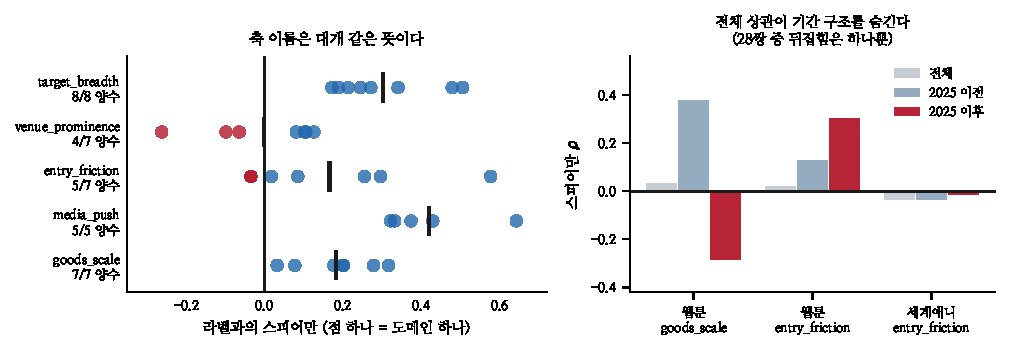
\includegraphics[width=\textwidth]{figs/hide.pdf}
\caption{왼쪽 --- 축별 라벨 부호. 점 하나가 도메인 하나, 세로선이 평균.
오른쪽 --- 전체 상관이 기간 구조를 숨긴다.}
\end{figure*}

\section{축 이름은 대개 같은 뜻이다}

노트 5가 다섯 축을 정의하고 열 도메인에 매긴 뒤로, ``\texttt{media\_push}가
팝업에서와 웹툰에서 같은 것을 재는가''를 한 번도 안 물었다. 프로크루스테스
정렬(노트 5--124)은 축이 \emph{다를} 것을 전제하고 회전으로 맞추는 장치였고,
직접 풀링(노트 125 이후)은 같을 것을 전제한다. 어느 쪽이 맞는지를 안 쟀다.

\begin{table}[t]
\centering\tsize
\caption{축과 라벨의 스피어만. 도메인 여덟(레코드 100건 이상).}
\begin{tabular}{lrr}
\toprule
& 양수 & $|r|$ 평균 \\
\midrule
target\_breadth & \textbf{8/8} & .303 \\
media\_push & \textbf{5/5} & .421 \\
goods\_scale & \textbf{7/7} & .184 \\
entry\_friction & 5/7 & .186 \\
venue\_prominence & 4/7 & .120 \\
\bottomrule
\end{tabular}
\end{table}

\claimx{\textbf{셋은 전 도메인에서 같은 방향이다.} \texttt{target\_breadth} ·
\texttt{media\_push} · \texttt{goods\_scale}이 예외 없이 양수다. 직접
풀링의 전제가 이 셋에서는 맞다.}{\texttt{venue\_prominence}는 4/7이고
$|r|$ 평균이 0.120으로 제일 약하다 --- 팝업에서는 물리적 장소인데 웹툰 ·
애니에서는 무엇으로 매겼는지 축 정의가 도메인마다 늘어나 있을 수 있다.}

\section{그런데 전체 상관이 거짓말을 한다}

노트 139에서 웹툰의 \texttt{entry\_friction} 하나로 $+$0.3009를 냈는데,
같은 축의 전체 상관은 $+$0.019다. 무관한 축이 어떻게 그만큼 예측하나.
기간을 갈랐다.

\begin{table}[t]
\centering\tsize
\caption{웹툰. 같은 축, 기간만 가른 것.}
\begin{tabular}{lrrr}
\toprule
& 전체 & 2025 이전 & 2025 이후 \\
\midrule
entry\_friction & $+$.019 & $+$.129 & \textbf{$+$.301} \\
\textbf{goods\_scale} & $+$.033 & \textbf{$+$.378} & \textbf{$-$.283} \\
\bottomrule
\end{tabular}
\end{table}

\claimx{\textbf{\texttt{entry\_friction}은 뒤집힌 게 아니라 강해진다.}
두 기간 다 양수이고 이후가 더 세다. 전체로 합치면 $+$0.019가 되는 것은
두 기간의 \emph{수준}이 달라 상쇄되기 때문이다.}{심슨의 역설의 한
형태다. 전체 상관을 축의 요약으로 쓰면 이런 구조가 통째로 안 보인다.}

\claimx{\textbf{\texttt{goods\_scale}은 진짜로 뒤집힌다} --- $+$0.378에서
$-$0.283으로. 도메인$\times$축 28쌍을 다 보니 \textbf{뒤집힘은 이 하나뿐}
(4\%)이다.}{``뒤집힘''을 양쪽 $|r|>0.10$이고 부호가 반대인 것으로
정의했다. 문턱을 낮추면 몇 쌍 더 나올 수 있다.}

\section{그 하나가 셋을 설명한다}

\begin{table}[t]
\centering\tsize
\caption{노트 138--139의 관측과 그 원인.}
\begin{tabular}{ll}
\toprule
관측 & 원인 \\
\midrule
웹툰 단독 $+$.246 $\to$ $-$.191 & goods\_scale 하나 \\
안쪽 창이 그 축을 1위로 & 안쪽 $=$ 이전 기간, $+$.378 \\
완결 플래그가 축 다섯을 이김 & 뒤집힌 축이 나머지를 덮음 \\
\bottomrule
\end{tabular}
\end{table}

\claimx{\textbf{세 관측이 한 뿌리다.} 웹툰 \texttt{goods\_scale}의 관계가
2025년에 반대가 됐고, 학습 기간 안쪽은 전부 이전이라 그 축이 제일 좋아
보이며, 그것을 쓴 모형이 이후에 무너진다. 완결 플래그가 이긴 것은 플래그의
관계가 안 뒤집혔기 때문이지 플래그가 더 나은 정보라서가 아니다.}{왜 뒤집혔는지는
모른다. 웹툰 라벨은 네이버 즐겨찾기이고 \texttt{goods\_scale}은 굿즈 규모인데,
웹툰에 굿즈 규모를 어떻게 매겼는지부터 다시 봐야 한다.}

\section{규약 하나}

\claimx{\textbf{축을 볼 때 전체 상관을 쓰지 않는다.} 앞으로 축의 요약은
기간을 가른 값으로 적는다. 노트 116의 후보 축 스물세 개도 전체 상관으로
걸렀는데, 그 문턱을 통과하거나 걸린 것 중에 이런 구조가 숨어 있을 수
있다.}{노트 117의 누수 가드는 $|$라벨 상관$| \ge 0.70$을 차단한다 --- 그
상관도 전체로 잰 것이다. 뒤집히는 축은 전체 상관이 0에 가까워 \emph{누수
가드를 그냥 통과한다.}}

반증 조건의 마지막 줄이 다음 할 일이다. 노트 116에서 잰 후보 축 스물세 개를
기간을 갈라 다시 보면, ``전체로는 약해서 안 쓴 축'' 중에 실은 두 기간 다
강한 것이 있을 수 있다.

\begin{table}[t]
\centering\tsize
\caption{남은 것.}
\begin{tabular}{ll}
\toprule
후보 축 23개 & 전체 상관으로 걸렀다 --- 기간 갈라 재검토 \\
goods\_scale & 웹툰에 어떻게 매겼나 \\
venue\_prom. & 4/7 · $|r|$ .12 --- 정의가 도메인마다 다른 듯 \\
\bottomrule
\end{tabular}
\end{table}

\end{document}
